%%%%%%%%%%%%%%%%%%%%%%%%%%%%%%%%%%%%%%%%%%%%%%%%%%%%%%%%%%%%%%%%%%%%%%%%%%%%%%%%%%%%%%%%%%
\section{Use Cases and Data Resources} \label{sect:motivation}                           %
%%%%%%%%%%%%%%%%%%%%%%%%%%%%%%%%%%%%%%%%%%%%%%%%%%%%%%%%%%%%%%%%%%%%%%%%%%%%%%%%%%%%%%%%%%

In this section, we briefly discuss a core use case for the ApiNATOMY application: the generation of interactive schematics in support of genomics and drug discovery studies. We introduce some of the key ontology- and data-resources required in this case. In so doing, we set the stage for an exposition of our early-stage results in the ApiNATOMY application effort.

The domains of genomics and drug discovery are heavily dependent on physiology knowledge, as both domains take into account the manufacture of proteins in different parts of the body and the transport of molecules that interact with those proteins, such as drugs, nutrients, and other proteins.
%%
We aim to provide an interactive, schematic overview of data resources important to these domains. This includes gene expression data (e.g.~\cite{EBI}), and data on the transport routes taken by molecular interactors (e.g.~\cite{HMC+13}). Such data may be usefully depicted in the form of a physiology \emph{circuitboard}.

In ApiNATOMY, a physiology circuitboard schematic consists of an \emph{anatomical treemap} and an overlay of \emph{process graphs}. Our earlier prototypes~\cite{BGS12,KBK14} presented treemaps of the Foundational Model of Anatomy (FMA) ontology~\cite{RM03}. Nesting of one treemap tile inside another indicated that the term associated with the child tile is either a mereotopological \emph{part} or a \emph{subclass} of the term associated with the parent tile. Our newest prototype also adopts this convention.

\begin{figure}%
	\centering%
	\begin{minipage}[b]{.52\linewidth}
		\centering%
		\subfigure[Initial view of ApiNATOMY]{
			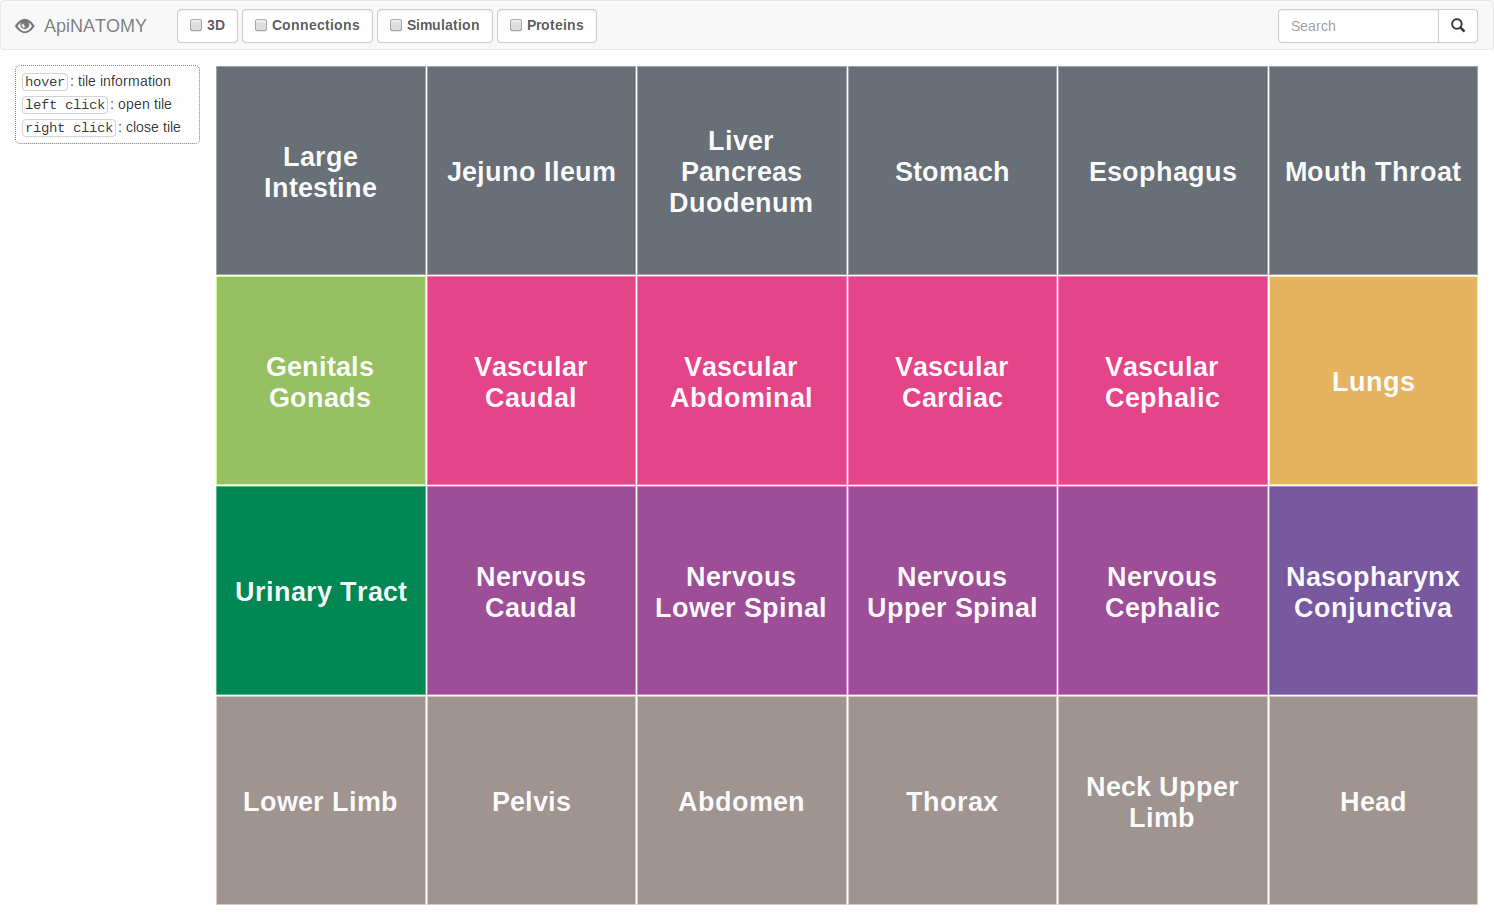
\includegraphics[width=\linewidth]{images/screenshot-main.png}
			\label{fig:24tiles}
		}
	\end{minipage}\hskip4mm
	\begin{minipage}[b]{.44\linewidth}
		\centering%
		\subfigure[Longitudinal section through the male human body, justifying the layout]{
			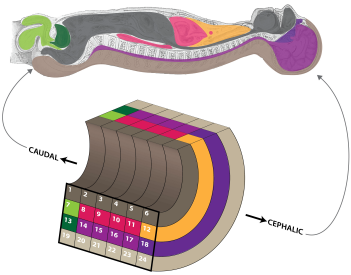
\includegraphics[width=\linewidth]{images/tilemap-cylinder.png}
			\label{fig:tilemap-cylinder}
		}
	\end{minipage}\vskip2mm
	\caption{The main 24-tile layout of the ApiNATOMY circuitboard}
	\label{fig:treemaps}
\end{figure}

The ApiNATOMY Graphical User Interface (\cref{fig:24tiles}) supports user interaction with circuitboard schematics via point-and-click navigation of the treemap content. The upper level of the anatomical treemap is arranged to resemble the longitudinal section through the middle of the human body (\cref{fig:tilemap-cylinder}). Each of the organs in the plan is composed of multiple tissues and sub-organs. The GUI supports data filtering across multiple levels and contextual zooming into selected areas.

This type of interaction extends also to the overlayed process graphs.
These graphs project routes of blood flow processes linking different regions of the human body ---using data generated in~\cite{deB11}---, as well as transport processes along neurons of the central nervous system (i.e., the brain and spinal cord) --- using data obtained via the Neuroscience Information Framework~\cite{Gar+08}.

The ApiNATOMY GUI is built from inception as a three-dimensional (3D) environment. This facilitates interaction not only with 3D renderings of the circuit boards themselves, but also with a wide range of geometry/mesh formats for volumetric models of biological structure across scales. For instance, it is already possible to overlay Wavefront \texttt{.obj} data from BodyParts3D~\cite{MFT+09} as well as \texttt{.swc} data provided by \texttt{neuromorpho.org}~\cite{Asc06}. Easy access to such visual resources is critical to the understanding of long-range molecular processes in genomics and drug discovery research.

In the next two sections, we discuss our techniques for (i) constraining treemap layouts to generate stable anatomical treemaps,
(ii) designing and overlaying physiological communication routes for the cardiovascular and neural systems,
(iii) querying and depicting protein architecture diagrams for the anatomical overview of gene expression data, and
(iiii) running simulations using mathematical models relevant to molecular mechanisms, and overlaying the results.
% TODO: Do we actually discuss (iiii) in this paper?

